% scusate, mi sono un po' rotto di continuare a cambiare lingua tra inglese e italiano, così ho deciso di riscrivere gli appunti per conto mio traducendo (con parecchi copia-incolla delle parti già in italiano)

\documentclass[a4page, 11pt]{article}

\usepackage{graphicx}
\graphicspath{ {./img/} }

\usepackage{hyperref} %clickable stuffs
\usepackage{mathtools}
\usepackage[margin=1.3in]{geometry}
\usepackage[utf8]{inputenc}
\usepackage[italian]{babel}
\usepackage[autostyle]{csquotes}
\MakeOuterQuote{"} %almost there, i removed `` everywhere to make it work better! D.
\usepackage{enumitem}
\usepackage[backend=biber]{biblatex}

\addbibresource{biblio.bib}


\title{Data Management}
\author{}
\date{}

\begin{document}
\maketitle

\tableofcontents
\newpage

\part{Modelli di dati}
Il \textit{data modelling} è uno strumento per descrivere parte del mondo reale, permettendo di immagazzinare dati in un database ed effettuare interrogazioni sfruttando un linguaggio creato ad hoc.
Il linguaggio di interrogazione deve essere comprensibile sia alla macchina che all'uomo, espressivo, semplice, flessibile e, se possibile, deve seguire degli standard.
Il modello di dati più famoso è quello relazionale (rappresentato da SQL).

I modelli di dati seguono il Teorema di CAP, introdotto da Eric Brewer nel 2000:
\begin{itemize}
\item Consistency: tutti i nodi vedono gli stessi dati allo stesso istante;
\item Availability: ogni nodo deve rispondere alle richieste rivoltegli;
\item Partition Tolerance: il sistema funziona anche con dati frammentanti su una rete di calcolatori.
\end{itemize}
È impossibile per un modello soddisfare contemporaneamente tutte e tre le caratteristiche\cite{NoSQLDB}.
Il modello relazionale segue le leggi CA, mentre i modelli NoSQL sono CP o AP (dipende dal modello).
Si tende a preferire la disponibilità alla coerenza per ottenere dati non aggiornati piuttosto che messaggi di errore.


\section{SQL.}
Nato negli anni '70, il modello relazionale è ben sviluppato e conosciuto e gode di un'ottima reputazione: è stato lo standard \textit{de facto} per anni ed è ancora considerato il migliore per garantire l'integrità dei dati (permessa dal suo schema rigido).
Il modello relazionale segue quattro proprietà rappresentate dalla sigla ACID:
\begin{itemize}
\item Atomicity: l'operazione è \textit{atomica}, ovvero o avviene per intero (\verb|COMMIT|) o restituisce un errore e il database ritorna alla forma iniziare (\verb|ROLLBACK|);
\item Consistency: i nuovi dati inseriti rispecchiano lo schema prestabilito (o l'operazione di inserimento fallisce);
\item Isolation: le singole operazioni non influiscono sulle altre; per fare questo il database costruisce una coda di esecuzione dei processi, così lo stato del database non muta durante l'esecuzione di una singola richiesta;
\item Durability: la persistenza del file è garantita (virtualmente a tempo indefinito) anche in caso di crash del sistema; per ottenere questo risultato sono utilizzati backup e log files.
\end{itemize}

Il modello relazionale tuttavia è fortemente influenzato dalla tecnologia degli anni in cui è nato: permette infatti di archiviare la maggior quantità di informazione occupando il minor spazio possibile su disco (allora gli hard disk erano costosi e ingombranti).
Nel tempo dunque si sono notati difetti nel modello:
\begin{itemize}[noitemsep]
\item un attributo può avere solo un tipo di valore;
\item SQL non è compatibile con i moderni linguaggi di programmazione ad oggetti;
\item la struttura del modello è molto rigida;
\item non permette loop nei dati;
\item la modifica di tabelle esistenti è difficile e dispendiosa.
\end{itemize}

Negli anni dunque si sono cercati modelli alternativi.
Nei RDBMS la performance (cioè la velocità di esecuzione) dipende da vari fattori:
\begin{itemize}
\item numero delle righe;
\item tipo di operazione;
\item algoritmo scelto;
\item struttura dei dati.
\end{itemize}

Inoltre il modello relazionale rende difficile scalare l'hardware: è stato pensato per poter girare su un'unica macchina fisica\footnote{Il modello \textit{NewSQL} proposto nel 2011 tenta di risolvere a questo inconveniente}.


\section{NoSQL.}
Per risolvere i problemi dei database relazionali, nasce un movimento informatico chiamato NoSQL (\textit{Not Only SQL}) che non rifiuta il modello ma propone approcci alternativi: i database NoSQL non hanno un modello prestabilito rendendo facile archiviare dati non strutturati e permettendo di aggiungere attributi senza modificare l'intero modello.
Mentre il modello relazionale si basa sull'assunzione del \textit{mondo chiuso}\footnote{\url{https://it.wikipedia.org/wiki/Ipotesi_del_mondo_chiuso}} (se il valore di verità non è noto, si considera la proposizione falsa), i modelli NoSQL adottano il modello del \textit{mondo aperto}\footnote{\url{https://it.wikipedia.org/wiki/Ipotesi_del_mondo_aperto}} secondo il quale non si può stabilire il valore di verità di cosa non è noto.

È possibile \textit{scalare} (\textit{scaling}) un DBMS potenziando l'hardware su cui è ospitato.
Si distingue lo scalare verticalmente (\textit{Scaling Up}), il potenziare la singola macchina, dallo scalare orizzontalmente (\textit{Scaling out}), aggiungere macchine in una rete di calcolatori; quest ultimo caso è molto difficile da effettuare su un database di tipo relazionale.
Il costo è un altro dei problemi: l'acquisto di macchine di una certa potenza è molto alto e non garantisce un aumento lineare delle prestazioni, che anzi scendono asintoticamente.

Opponendosi alla rigidità del modello relazionale, le proprietà dei database NoSQL non potevano che essere riassunte dall'acronimo BASE:
\begin{itemize}
\item Basic Availability: la consistenza può anche non essere garantita interamente, mostrando solamente una parte dei dati realmente disponibili (è il tipico caso di crash di un nodo che quindi non può trasmettere i dati al resto della rete);
\item Soft State: i dati possono avere schemi diversi (a differenza del modello relazionale);
\item Eventual Consistency: i sistemi NoSQL richiedono che, ad un certo punto, i dati convergano a uno stato consistente senza specificare quando; prima del raggiungimento della consistenza si possono avere valori non veritieri.
\end{itemize}

\begin{center}
\begin{tabular}{l|l}
ACID & BASE \\
\hline
Forte Coerenza & Coerenza debole \\
Poca disponibilità & Forte disponibilità \\
Difficilmente scalabile & Facilmente scalabile\\
Rigido & Flessibile \\
\end{tabular}
\end{center}

I modelli NoSQL si dividono in quattro macro categorie\cite{NoSQLDB, GraphDB}:
\begin{enumerate}[noitemsep]
\item Document based (CouchDB, MongoDB): di solito salvati con file JSON, contenente un insieme ordinato di coppie \textless{}chiave - valore\textgreater{}; è facile ricercare dati in questo formato;
\item Graph based (Neo4J, FlockDB): sfrutta il concetto matematico di grafo per archiviare i dati come nodi ed esaltare i legami tra di essi costruendo archi; è difficile da scalare per quanto riguarda l'immagazzinamento (è difficile tagliare un grafo) ma è molto rapido nelle query.
\item Key Value (Dynamo, Voldemort, Rhino DHT): sono delle tabelle di coppie \textless{}chiave - valore\textgreater{} con chiavi che si riferiscono (o puntano) a un certo dato, è molto simile ai Document based.
\item Column family (Big Table, Cassandra): sono tabelle sparse e annidate contenenti coppie \textless{}chiave - valore\textgreater{}, sono in grado di salvare grandi quantità di dati.
\end{enumerate}

Costando di meno lo spazio di archiviazione, questi modelli non tentano di minimizzare lo spazio occupato su disco ma puntano a massimizzare le prestazioni nelle operazioni di R/W.
La ridondanza dei dati facilita questo compito pur aumentando notevolmente le dimensioni dei dati stessi: si sacrifica spazio di archiviazione a favore della velocità di lettura.
La semplicità del modello permette di archiviare un maggior numero di dati:
\begin{center}
	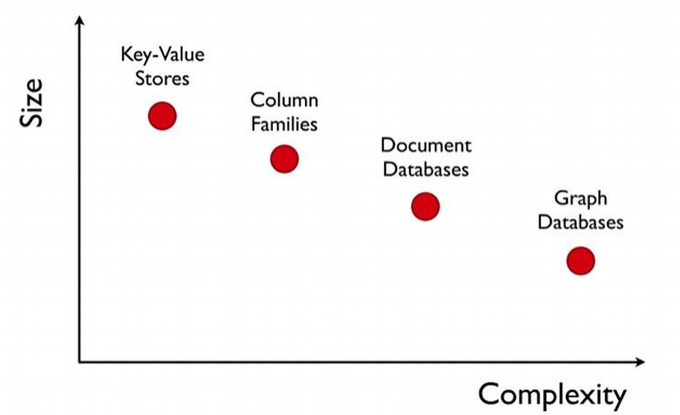
\includegraphics[scale=0.4]{IMAGE1.jpg}
\end{center}


\subsection{Document Based: MongoDB\cite{MongoDB, ScalingMongoDB}.}
MongoDB è, come già affermato, un sistema di gestione basato sui documenti (\textit{Document Based Management System}), in cui i dati sono archiviati in formato BSON (Binary JSON) e letti tramite indici.
MongoDB non prevedere operazioni di join.
Cambiano i nomi delle entità rispetto al modello relazionale:
\begin{center}
  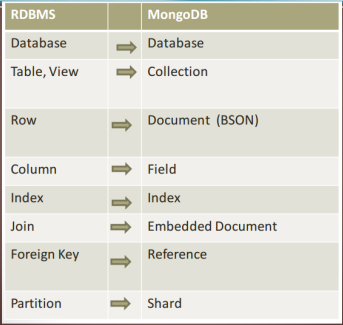
\includegraphics[scale=0.6]{IMAGE2.jpg}
\end{center}

Lavorando su una rete di calcolatori, MongoDB può impiegare un tempo considerevole a importare documenti da un database preesistente; nel caso in cui si si voglia velocizzare il processo, si potrebbe decidere di apportare alcune modifiche:
\begin{itemize}[noitemsep]
\item disabilitare il riconoscimento dei dati, che è un segnale trasmesso tra processi di comunicazione, computer o dispositivi, per indicare il riconoscimento o la ricezione del messaggio, come parte di un protocollo di comunicazione;
\item disabilitare la scrittura su un file di tipo log che ha funzione di backup.
\end{itemize}
Bisogna stare molto attenti nel fare ciò, perché ogni ogni perdita non sarà registrata e di conseguenza sarà definitiva.
\newline

Per dataset di grandi dimensioni risulta molto utile l'utilizzo di indici: simili agli indici dei libri (o delle tabelle SQL), rappresentano un modo più veloce per recuperare informazioni.
L'uso di indici rallenta l'inserimento di nuovi dati (perché appunto devono essere indicizzati) ma velocizza notevolmente le ricerche.
Il campo \verb|_id| è sempre indicizzato.
Senza un indice, MongoDB analizza a tappeto tutti i documenti (esattamente come SQL).
Metaforicamente dovrebbe leggere ogni volta tutto il libro per recuperare l'informazione.
L'indicizzazione evita proprio questo problema (che aumenta con le dimensioni della \textit{collection}) organizzando il contenuto in una lista ordinata.
Dato che l'indicizzazione rallenta le modifiche, è buona norma utilizzare solamente un paio di indici per ogni collection; il limite di MongoDB è di 64 indici.
Il comando è il seguente:
\begin{verbatim}
db.<collection>.ensureIndex({
  <field1> : <sorting>,
  <field2> : <sorting> ...
});
\end{verbatim}
dove \verb|<sorting>| assume il valore $+1$ per ordinamenti in ordine crescente e $-1$ per ordine decrescente.
I campi \verb|field| devono essere presenti in tutti i documenti della collection.

È possibile effettuare una sorta di \verb|join| in MongoDB grazie all'algoritmo \textit{pipeline}\cite{NoSQLDB}, che però impiega più tempo del corrispettivo SQL.
Pipeline permette di eseguire operazioni di \verb|$match| e \verb|$group| su una collection così da eseguire una operazione su insiemi di risultati.
\begin{center}
  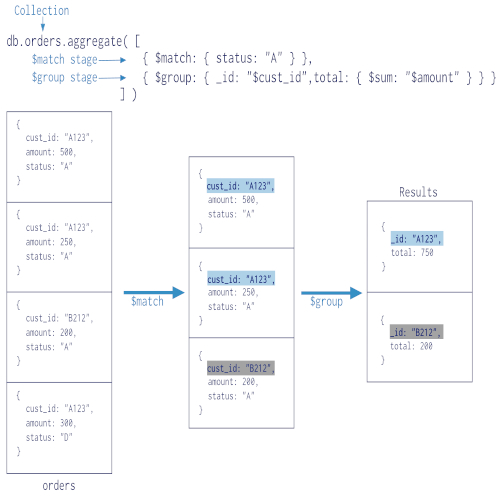
\includegraphics[scale=0.6]{mongodb-pipeline.jpg}
\end{center}

Per ragioni commerciali, MongoDB offre anche un'interfaccia SQL tramite il connettore BI (Business Intelligence): genera lo schema relazionale e lo usa per accedere ai dati.


\subsection{GraphDB: Neo4J\cite{GraphDB}.}
Un grafo è una collezione di nodi e archi, i quali rappresentano le relazioni tra i nodi stessi.
È facile modellare numerose realtà, come: social media, raccomandazioni, luoghi geografici, reti logistiche, grafici per le transazioni finanziarie (per il rilevamento delle frodi), master data management, bioinformatica, sistemi di autorizzazione e controllo degli accessi.
Il modello a grafo con etichette (\textit{labeled-property graph model}) ha le seguenti caratteristiche:
\begin{itemize}[noitemsep]
\item contiene \textit{nodi} e \textit{relazioni};
\item i nodi contengono \textit{proprietà} (coppie \textless{}chiave-valore\textgreater{});
\item i nodi possono essere etichettati con una o più \textit{etichette};
\item le relazioni sono nominali e direzionali, con un nodo d'inizio e uno di fine;
\item le relazioni, come i nodi, possono avere delle proprietà (e queste possono avere anche valori).
\end{itemize}
Le proprietà delle relazioni possono essere assegnate con un criterio \textit{fine-grained} o \textit{generic}.
Considerando il caso della relazione \verb|ADDRESS|, si può fare distinzione tra:
\begin{itemize}
\item fine-grained: \verb|HOME_ADDRESS|, \verb|WORK_ADDRESS| o \verb|DELIVERY_ADDRESS| (sono tutte etichette diverse);
\item generic: \verb|ADDRESS:home|, \verb|ADDRESS:work| o \verb|ADDRESS:delivery| (l'etichetta è sempre \verb|ADDRESS|, con un valore che ne indica il tipo).
\end{itemize}
Generalmente è preferito il secondo metodo per la minore complessità nello scrivere query (come ad esempio elencare tutti gli indirizzi di una data persona).

Un database a grafo può usare un motore di archiviazione nativamente a grafo o usare altri sistemi di archiviazione.
Il primo ottimizza la gestione dei grafi, mentre il secondo archivia i dati in formato tabellare o tramite documenti per poi interrogare il database come se fosse un grafo.
Il metodo tabellare per esempio archivia le relazioni su una tabella relazionale che può essere interrogata tramite \textit{join bomb} (join con se stessa), tuttavia questo sistema degenera in fretta all'aumentare della distanza tra due nodi.

Il database a grafo risolve quindi il problema dei database relazionali (e di molti altri database NoSQL) a gestire le relazioni interne ai dati.
Infatti anche altri modelli NoSQL, indipendentemente dal modello adottato, soffrono perdite di prestazioni quando sono effettuate aggregazioni (soprattutto non indicizzati) dal momento che i collegamenti non sono nativi e manca il concetto di prossimità, presente invece nel grafo.
Si può tentare di risolvere il problema con dati annidati tra di loro ma la struttura del database risulterebbe eccessivamente complessa e non permetterebbe altre query.
Il DBA in base ai suoi bisogni (integrazione con altre applicazioni) può benissimo decidere di usare un database a grafo con una gestione dei dati non nativa senza che questo impatti sulla qualità del prodotto finale.
In un archivio nativo a grafo gli attributi, i nodi e i nodi referenziati sono memorizzati insieme per ottimizzare l'engine l'elaborazione a grafo.

Per eseguire una query nel modello a grafo, il tempo di risposta non dipende strettamente dal numero totale di nodi (che rimane più o meno costante) perché la query viene processata nella porzione locale del grafo connessa al nodo base, mentre nei modelli relazionali e altri modelli NoSQL le prestazioni calano al aumentare dei dati (spesso in una maniera lineare).
Inoltre è possibile aggiungere altri nodi e relazioni senza disturbare il modello già esistente anche nel caso in cui i dati non abbiano la stessa struttura.
Il processing engine usa \textit{``index-free adjacency''} cioè i nodi connessi sono collegati fisicamente tra di loro, ciò velocizza il loro recupero da una query, ma questa velocità ha un prezzo: l'efficacia delle query che non sfruttano le proprietà del grafo viene peggiorata, ad esempio nel caso delle operazioni di R/W.

Neo4j implementa un linguaggio Cypher, di tipo dichiarativo, che permette query al grafo usando una sintassi simile a SQL o SPARQL, ma comunque ottimizzata per i grafi.
Cypher è facile da leggere e capire ed espressivo, pur rimanendo compatto.
Il linguaggio astrae il concetto di grafo permettendo all'autore di una query di indicare solamente cosa desidera tralasciando come. \newline
Neo4J utilizza in parallelo il linguaggio Gremlin, parte del framework Apache TinkerPop, che invece permette di esplicitare le modalità con cui deve essere svolta una richiesta al database.


\subsection{Key-Value.}
Considerato il modello più semplice e flessibile, associa ad una stringa (la \textit{chiave}) una sequenza di dati binari (BLOB, \textit{Binary Large OBject}) come possono essere immagini, video o altri tipi di dato:
\begin{center}
  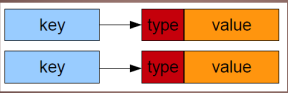
\includegraphics[scale=0.5]{IMAGE3.jpg}
\end{center}
Le uniche operazioni lecite del modello sono;
\begin{itemize}
\item aggiunta di una nuova coppia \textless{}chiave - valore\textgreater{};
\item rimozione di una coppia \textless{}chiave - valore\textgreater{};
\item modifica di un valore (data la chiave);
\item ricerca di un valore (data la chiave).
\end{itemize}
Data la natura \textit{opaca} dei dati, non è possibile cercare la chiave dato il valore.

Esempi noti di Database key-value sono DynamoDB, sviluppato e usato da Amazon per registrare i sistemi di pagamento dei clienti, e Riak, che usa la seguente terminologia:
\begin{center}
  \begin{minipage}[b]{0.4\textwidth}
    \begin{tabular}{|l|l|}
      \hline
      \textbf{SQL} & \textbf{Riak}\\ \hline
      database & cluster \\ \hline
      table & bucket \\ \hline
      row & key-value\\ \hline
      rowid & key\\ \hline
    \end{tabular}
  \end{minipage}
  \begin{minipage}{.5\textwidth}\centering
    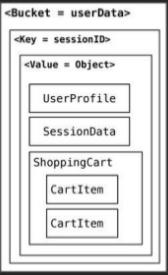
\includegraphics[scale=0.6]{IMAGE4.jpg}
  \end{minipage}
\end{center}

Grazie all'indicizzazione ad \textit{hash}, questo modello riesce a scalare orizzontalmente in modo molto efficiente.
L'hash è una funzione matematica che assegna un valore ad una chiave: $h(x) = v$; nel caso specifico, generalmente il valore della funzione indica dove il dato si trova (non il dato stesso).
I valori hash possono essere facilmente distribuiti su una rete di calcolatori di dimensione arbitraria: per esempio, considerando la funzione $h(x) = x \% k$ (dove $\%$ è la funzione resto della divisione intera e $k$ il numero di nodi della rete), si può stabilire in quale nodo indirizzare la coppia in base al risultato.
Per recuperare il dato, basta dunque interrogare il nodo in cui è presente la chiave e attendere che questo invii il valore.


\subsection{Wide Column: Cassandra\cite{Cassandra} e BigTable.}
L'idea di archiviare i dati per colonne è nata negli anni '70, ma le prime implementazioni commerciali del modello risalgono solamente agli anni '90; di notevole importanza sono BigTable, introdotto da Google e da cui nasce Apache HBase, e Cassandra, sviluppato da Facebook.
Questo modello archivia i dati, raggruppati per colonne, su blocchi sequenziali dell'hard disk.
Questo ottimizza le aggregazioni della colonna e le query eseguite su più colonne (il tempo dipende comunque da eventuali indicizzazioni e dal design del database).
In un certo senso, questo modello è un'evoluzoine del KeyValue: quando si tenta di apportare una struttura al valore indicizzato dalla chiave, si ottiene un risultato simile (a tal punto che Cassandra può essere considerato un KeyValue).
Questo modello offre prestazioni elevate scalando orizzontalmente, quando sono richieste numerose operazioni di R/W al secondo su grosse quantità di dati e quando è necessario avere indicazioni temporali riguardanti ogni dato.
Si può usare anche costruire un database ibrido tra questo modello e quello a grafo: nascono così progetti come JanusGraph.
Il modello non permette join, ma si può ottenere un equivalente grazie alle funzioni \verb|Scan()| e \verb|Get()|.

\subsubsection*{BigTable e HBase.}
Sviluppato da Google, BigTable gestisce i dati costruendo delle mappe multidimensionali, ordinate, persistenti e sparse, accessibili grazie ad un indice di riga, ad un indice di colonna e a un \textit{timestamp}.
Ogni tabella è composta da \textit{column-families}, le cui celle sono ordinate e sparse (ovvero contengono chiavi diverse).
Si può rappresentare la struttura nel seguente modo:


\begin{center}
  \begin{tabular}{|c|c|c|}
    \hline
    \textbf{row key} & \textbf{column family 1} & \textbf{column family 2} \\
    \hline
                     &
                       \begin{tabular}{l|l}
                         \textbf{column 1} & \textbf{column 2} \\
                         \hline
                       \end{tabular}
                     &
                       \begin{tabular}{p{1.8cm}|p{1.8cm}|p{1.8cm}}
                         \textbf{column 1} & \textbf{column 2} & \textbf{column 3} \\
                         \hline
                       \end{tabular} \\
                       % \hline
    \textbf{KEY}
                     &
                       \begin{tabular}{l|l}
                         \textit{cell} & \textit{cell}
                       \end{tabular}
                     &
                       \begin{tabular}{p{1.8cm}|p{1.8cm}|p{1.8cm}}
                         \textit{cell} & \textit{cell} & \textit{cell}
                       \end{tabular} \\
    % \hline
                     &
                       \begin{tabular}{l|l}
                         \textit{cell} & \textit{cell}
                       \end{tabular}
                     &
                       \begin{tabular}{p{1.8cm}|p{1.8cm}|p{1.8cm}}
                         \textit{cell} & \textit{cell} & \textit{cell}
                       \end{tabular} \\
    \hline
  \end{tabular} \\
  ~\\
  Ogni riga può avere un timestamp diverso, quindi si possono avere più versioni della stessa tabella.
\end{center}

I dati all'interno della cella (e la chiave) non hanno tipo ma sono salvati come sequenza di byte, quindi per cercare un dato nota la chiave è necessario usare una funzione \verb|.toBytes("Key")|.
Le colonne sono dinamiche: è sempre possibile aggiungere una nuova colonna o modificare quelle esistenti (anche grazie ad API esterne).
Ogni colonna può appartenere ad una sola column-family e appartiene alla riga con \verb|familyNode:columnName| seguito dal valore:
\begin{verbatim}
row-key : {
    info : {
        height : 170,
        state : "NY"
    },
    roles : {
        ASF : "Director",
        Hadoop : "Founder"
    }
}
\end{verbatim}
Il numero di versione per ogni riga è univoco per ogni row-key: generalmente è usato un timestamp, ma può essere modificato dall'utente.

\subsubsection*{Cassandra.}
Nato come supporto per la ricerca nell'inbox di Facebook, fu reso open source nel 2008 e in seguito è diventato un top-level project sotto Apahe nel 2010.
Il modello è identico a quello di BigTable e HBase con alcune differenze per gli algoritmi utilizzati e il modo in cui i dati sono distribuiti.
Usa un linguaggio chiamato CQL (Cassandra Query Language) simile a SQL.

Il \textit{Keyspace}, che sarebbe l'equivalente del database in un RDBMS, possiede nativamente un fattore di replicazione e un algoritmo di replicazione, ma rimane solamente un raggruppamento di column families.
\begin{center}
	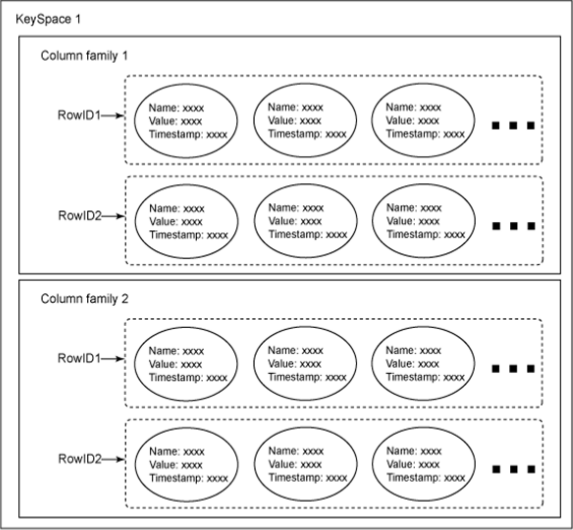
\includegraphics[scale=0.5]{IMAGE5.png} \newline
	An example of Cassandra data model.
\end{center}

Non permettendo operazioni di join o chiavi esterne, il modello prevede l'uso di dati ridondanti e denormalizzati per gestire i collegamenti.

\subsubsection*{Confronto tra i tre DBMS WideColumns.}
\begin{center}
  \begin{tabular}{l|l|l|l}
    & \textbf{Cassandra} & \textbf{Big Table} & \textbf{DynamoDB} \\
    \hline
    \textit{Tipologia:} & Column & Column & Key-Value \\
    % \hline
    \textit{Progettato per:} & Write often, read less & Large scalability & Large database \\
    % \hline
    \textit{Gestione parallela:} & MVCC & Locks & ACID \\
    % \hline
    \textit{Consistency:} & & Sì & Sì \\
    \textit{Hight Availability:} & Sì & Sì & Sì \\
    \textit{Partition Tolerance:} & Sì & Sì & \\
    \textit{Persistenza:} & Sì & Sì & \\
  \end{tabular}
\end{center}


\part{Distribuzione dei dati}
Un database centralizzato è un sistema in cui il database è localizzato su una sola macchina: se questa non è funzionante (SPOF, \textit{Single Point of Failure}), l'intero database non risulta accessibile.
Per facilitare l'accesso ai dati in luoghi differenti, è possibile distribuirli o replicarli: nel primo caso si distribuiscono in luoghi diversi dati diversi, nel secondo i medesimi dati (per intero o solamente in parte).
La distribuzione permette una maggiore disponibilità (\textit{availability}) e la parallelizzazione delle operazioni.
In fase di progettazione di un Database Distribuito, si costruisce la rete tra i nodi, si collocano questi geograficamente e si stabilisce il loro contenuto.
Le macchine su cui gira un database distribuito non sono particolarmente potenti: si riduce notevolmente il costo dell'hardware ma la progettazione risulta più difficile.
Bisogna tenere presente però che la prestazione totale di un database distribuito è, generalmente, pari alla prestazione del nodo più debole: è il fenomeno \textit{bottleneck}.
Le performance tuttavia migliorano linearmente rispetto al numero di nodi della rete, ma risultano influenzate dalla velocità di connessione.

In un Database Distribuito Omogeneo, tutti i \textit{nodi} condividono le medesime impostazioni (non è possibile individuare una gerarchia): insieme collaborano a risolvere le richieste dell'utente, a cui appare come un singolo sistema.
Invece in un Database Distribuito Eterogeneo i nodi hanno impostazioni diverse, rendendo difficili le comunicazioni per risolvere query e altre transazioni, che sono risolte limitatamente alla loro parte.

Un sistema distribuito tiene in memoria, nel complesso della rete, una copia di ogni dato su un numero di nodi stabilito dal \textit{replication factor}.
Ciò garantisce una maggiore tolleranza agli errori (è più difficile avere un SPOF): il dato è ottenibile da più fonti diverse, dunque se un nodo non è disponibile la rete gira la richiesta ad un altro.
Inoltre la replicazione del database migliora con la sua frammentazione: i nodi replicano i dati spartendosi i frammenti (\textit{churn}), riducendo le comunicazioni interne.
In questo modo si possono distribuire le richieste ai singoli nodi, che elaborano in parallelo e inviano all'utente il risultato.

Tuttavia replicazione e frammentazione rischiano di compromettere la coerenza del dataset: sono da considerare il tempo di aggiornamento di ogni replica e la gestione di operazioni contradditorie eseguite parallelamente (ad esempio, l'acquisto contemporaneo di due persone dell'ultimo biglietto per un volo aereo).
Per ovviare a questo problema, una possibile soluzione è costruire una struttura gerarchica all'interno dei nodi: si individuano \textit{master} che interagiscono con l'utente e \textit{slaves} che hanno una mera funzione di replica (a meno che il rispettivo \textit{master} non sia disponibile).

\section{Frammentazione.}
La frammentazione dei dati invece avviene dividendo i dati in $k$ parti in modo tale preò che sia possibile ricostruire la relazione originaria.
La frammentazione può essere orizzontale (si dividono le osservazioni) o verticale (si dividono gli attributi) in base alla struttura del modello.
In ogni caso dovrebbe garantire che i dati siano presenti nei nodi che li processano più frequentemente; inoltre è permessa così la parallelizzazione dei processi (per osservazioni o per caratteristiche).
Si possono anche avere frammentazioni ibride.

Si intende con \textit{Data Transparency} la consapevolezza che ha l'utente finale della distribuzione dei dati: l'obiettivo è di far credere che si operi su un unico server. \newline

Si individuano tre tipologie di architetture nei DDBMS (\textit{Distributed DBMS}):
\begin{itemize}
\item \textit{Share Everything}: è un sistema centralizzato con un'unica macchina e (virtualmente) un unico disco;
\item \textit{Share Disk}: i dati sono archiviati su diversi dischi connessi tra loro a cui accedono diverse macchine;
\item \textit{Share Nothing}: le macchine non condividono risorse ma operano all'interno di una rete (facile da scalare) sfruttata per unire i risultati.
\end{itemize}


\begin{center}
  \begin{tabular}{r|l}
    \textbf{Shared Disk} & \textbf{Shared Nothing} \\
    \hline
    Migliore gestione del carico di lavoro & Opera su \textit{commodity hardware}  \\
    High Availability & Facilmente scalabile \\
    Performance migliori con letture frequenti & Performance migliori con grossi volumi (R/W) \\
    I dati non sono partizionati & I dati sono partizionati in cluster
  \end{tabular}
\end{center}

\section{Replicazione.}
Si individuano diverse strutture di replica:
\begin{itemize}
\item One2Many: una sorgente e più repliche;
\item Many2One: più sorgenti e una sola replica (contenente tutti i dati);
\item Peer2Peer: i dati sono replicati attraverso molteplici nodi che comunicano l'uno con l'altro;
\item Bi-directional: un Peer2Peer a coppie;
\item Multi-Tier Staging: la replicazione è divisa in più stages.
\end{itemize}

Per creare una replica bisogna avere accesso alla porzione di dati da replicare: è necessario prelevare i dati dal nodo o usare un backup come sorgente.
Per sincronizzare le repliche durante l'operazione di trasferimento, si usano dei \textit{log file}: sequenze di attivitià realizzate, in ordine cronologico, che possono tenere conto delle transazioni (\textit{operations}) o di eventi di sistema (\textit{checkpoint} e \textit{dump}).
Si definisce \textit{checkpoint} un insieme di transazioni svolte in un determinato intervallo di tempo, mentre un \textit{dump} è una copia dello stato del Database in un dato istante temporale.


\newpage
\printbibliography[title={Letture di approfondimento}]
\end{document}